\documentclass[12pt]{IEEEtran}
\usepackage{colortbl}
\usepackage{booktabs}
\usepackage{subcaption}
\usepackage{algorithm}
\usepackage{algorithmicx}
\usepackage{algpseudocode}
\usepackage{tabulary}
\usepackage{pdfpages}
\usepackage{bigstrut}
\usepackage{graphicx}
\linespread{1}
\setlength\fboxsep{1pt}
\setlength\fboxrule{1pt}
\usepackage{multicol}
\usepackage{multirow}
\bstctlcite{IEEEexample:BSTcontrol}
\usepackage{multicol}
\usepackage{picture}
\newcommand{\quart}[4]{\begin{picture}(50,3)
{\color{black}\put(#3,3){\circle*{3}}\put(#1,3){\line(1,0){#2}}}\end{picture}}
\usepackage{amsmath}
\usepackage{balance}
\usepackage{flushend}
\usepackage[english]{babel}
\usepackage{blindtext}
\usepackage{times}
\usepackage{cite}
\usepackage{hyperref}
\hypersetup{
  colorlinks = false,
  hidelinks = true
}
\newcommand{\bi}{\begin{itemize}}
  \newcommand{\ei}{\end{itemize}}
\newcommand{\be}{\begin{enumerate}}
  \newcommand{\ee}{\end{enumerate}}
\newcommand{\tion}[1]{\textsection\ref{sec:#1}}
\newcommand{\fig}[1]{Figure~\ref{fig:#1}}
\setlength{\parindent}{0em}
\setlength{\parskip}{0.5em}
\usepackage[table,xcdraw]{xcolor}

\begin{document}
  \markboth{CSC 712: Software Testing and Reliability. Spring, 
    2015}%
  {CSC 712 Software Testing and Reliability. Spring, 
    2015}
  
  \title{On Strategies for Improving Software Defect Prediction}
  \author{Rahul Krishna, 
    \IEEEauthorblockA{\normalsize {\textit{Dept. of Electrical and Computer 
          Engineering}\\
        North Carolina State University, Email: 
        \href{mailto:rkrish11@ncsu.edu}{{rkrish11@ncsu.edu}}}}}
 \maketitle 
%  \IEEEcompsoctitleabstractindextext{%
    \begin{abstract}
      Programming inherently introduces defects into programs, as a result software systems can crash or fail to deliver an important functionality. It is very important to test a software throughly before it can be used. But an extensive testing can be prohibitively expensive or may take too much time to conduct This necessitates the use of automated software defect prediction tools. Although numerous machine learning algorithms are available to detect defects in software, but several factors undermine the accuracy of such algorithm. This paper uses Classification and Regression Trees (CART) and Random Forests to examines two approaches to counter the aforementioned problem. The first approach involves the use Synthetic Minority Oversampling Technique (also known as SMOTE). The second approach attempts to use a metaheursitic algorithm such as differential evolution to find the right set of parameters that can change the performance of the predictor. 
    \end{abstract}
    
    \begin{IEEEkeywords}
      Defect Prediction, Differential Evolution, CART, Random Forest, SMOTE.
    \end{IEEEkeywords}
%    }
%\maketitle

\section{Introduction} \label{intro}
Defect prediction is the study of identifying which software \textit{modules} are defective. Modules refer to some premitive units of an operating systems, like funtions or classes. It needs to be pointed out that early identification of possible defects can lead to a significant reduction in construction costs. No software is developed in a single day, or by just one person, rather it is constructed over time with old modules being extensively reused. Therefore, the sooner defects can be detected and fixed, the less rework is required for development. Boehm and Papaccio~\cite{boehm88} for instance mention that reworking software early in its life-cycle is far more cost effective (\textit{by a factor of almost 200}) than doing so later in it's life cycle. This effect has also been reported by several other studies. In their study, Shull \textit{et al.}~\cite{shull2002we} report that finding a repairing severe software defects is often hudereds of times cheaper if done during the requirements and design phase than doing so after the release. In fact, they claim that \textit{``About 40-50\% of user programs enter use with
  nontrivial defects.''}. Authur \textit{et al.} \cite{arthur99} conducted a controlled study with a few engineers at NASA's Langley Research Center, they found the group with a specialized verification team found, (a) More issues, (b) Found them early, which directly translates to lower costs to fix, see~\cite{dabney2006predicting}. 

All this leads use to one key conclusion: \textit{Find Bugs Early!} For this we need efficient code analysis measures. We also want them to be generic in that they must be applicable across several projects. Moreover, platforms such as github has over 9 million users, hosting over 21.1 million repositories. Faced with such a massive code base we need these to also be easy to compute. Static code measure is one such tool, it can automatically extracted from a code base with very little effort even for very large software systems~\cite{nagappan2005static}. Such measures reduce the effort required for defect prediction. As \cite{tosun2010ai} and \cite{ostrand2004bugs} have shown, if inspection teams used defect predictors to identify  issues, they can find 80\% to 88\% of the defects after inspecting only 20\% to 25\% of the code. With these code analysis measures, we can make use of classification tools form machine learning, such as CART and Random Forest, to detect the presence of defects. However, notice the skewness in the above result, \textit{ 80\% of the problems reside in only 20\% of the modules}. This is a key difficulty often faced in software defect prediction. In other words we are trying to predict the occurrence of a defect in a software most of whose modules work just fine. Therefore the classification tool that is used is quite often unable to detect the faulty modules. This is a very well known issue faced by several machine learning experts and is referred to as class imbalanced in datasets. A data set that is heavily skewed toward the majority class will sometimes generate classifiers that never predict the minority class. In software defect prediction, this bias often makes the classifier highly accurate in predicting non-defects, and totally useless for predicting defects.

One of the other issues in data mining is the choice of parameters that run these classification tools. The parameters of these data miners are rarely tested for the application they are being applied for. A common notion among it's users is that the space of options for these parameters has been well explored by experts and the best settings have been used. This is not necessarily true and that brings us to the research question that this paper tries to answer:
\begin{itemize}
\item[] {\bfseries RQ1:  Can over/under sampling techniques such as SMOTE to improve prediction accuracy for defect prediction?}
\item[] {\bfseries RQ2: Does Tuning a data miner improve it's prediction accuracy?}
\item[] {\bfseries RQ3: Is tuning performed in conjunction with SMOTE any better than either one performed alone?}
\item[] {\bfseries RQ4: Is the SMOTE\textit{ing} technique limited only to defect prediction?}
\end{itemize}



The rest of this paper is organized as follows--- Section \ref*{motivation} offers a small ilustration of the impact of SMOTE and tuning on the accuracy of the predictor. Section \ref*{back} highlights the underlying principles used in this paper. Section \ref{setup} presents the experimental setup followed by section \ref{expt} which presents the experimental results and discuss each one. Section \ref{concl} contains concluding remarks and finally section \ref{future} talks about the future work.\\[-1cm]

\begin{figure}[tbp!]
	
	{\footnotesize 
		\begin{tabular}{|p{0.95\linewidth}|}\hline\\[-0.3cm]
			\rowcolor[HTML]{FFFFFF}
			\begin{itemize}
				\item Statistical classifiers:
				Linear    discriminant analysis,
				Quadratic discriminant analysis,
				Logistic regression,
				Naive Bayes,
				Bayesian networks,
				Least-angle regression,
				Relevance vector machine,
				
				\item \textit{Nearest neighbor methods:} k-nearest neighbor, K-Star
				
				\item {\em Neural networks:} Multi-Layer Perceptron, Radial bias functions,
				
				\item \textit{Support vector machine-based classifiers:}
				Support vector machine,
				Lagrangian SVM
				Least squares SVM,
				Linear programming,
				Voted perceptron,
				
				\item \textit{Decision-tree approaches:}
				C4.5,
				CART,
				Alternating DTs
				\item \textit{Ensemble methods:}
				\textbf{Random Forest},
				Logistic Model Tree.
			\end{itemize}\\\hline
		\end{tabular}}
		\caption{Software Defect Predictors}\label{fig:lessmann}
	\end{figure}


\section{Background Notes}
\label{back}

This section briefly highlights the essential tools and methodologies discussed in this paper. Topics include Defect Prediction and Tuning with Differential Evolution.
\subsection{Defect Prediction}
The previous section presented key finding from literature that seem to conclude that defect prediction is quite important. This section introduces the idea of using instance based approach to identify defects. Assessing the quality of solutions to a real-world problem can be extremely hard~\cite{menzies2005xomo}. In several software engineering applications, researchers have models that can emulate the problem, for instance there is the COCOMO effort model~\cite[p29-57]{boehm2009software}, the COQUALMO defect model~\cite[p254-268]{boehm2009software}, Madachy’s schedule risk model~\cite[p284-291]{boehm2009software}, to name a few. Using these models it is possible to examine several scenarios in a short period of time, and this can be done in a reproducible manner. However, models aren't always the solution, as we shall see. 

There exist several problems where models are hard to obtain, or the input and output are related by complex connections that simply cannot be modeled in a reliable manner, or generation of reliable models take prohibitively long~\cite{Ludewig2003}. Software defect prediction is an excellent example of such a case. Models that incorporate all the intricate issues that may lead defects in a product is extremely hard to come by. Moreover, it has been shown that models for different regions within the same data can have very different properties \cite{localvsglobal}. This makes it extremely hard for one to design planning systems that are capable of mitigating these defects.

An alternative is the use of an instance based approach, an subset of case based reasoning strategy, instead of the conventional model based approach. Instance based approaches are used extensively by the effort estimation community. For more reference, see ~\cite{keung2008analogy, 6600685, walkerden1999empirical, shepperd1997estimating, kocaguneli2010use}. This approach has been proposed as an alternative to closed form mathematical models or other modeling methods such as regression \cite{keung2008analogy}. There are several other reasons for instance based approaches being a useful tool, see~\cite{6600685}. As pointed out by~\cite{walkerden1999empirical} it can be used with partial knowledge of the target project at an early stage which could be a very useful tool in preventing software defects. Instance based approaches are also rather robust in handling cases with sparse samples \cite{1438374}. All these features are desirable and suggest that instance-based approach is a useful adjunct to traditional model based approach. 
 
A recent IEEE TSE paper by Lessmann et al.~\cite{lessmann} compared 21 different learners for software defect prediction, listed in figure \ref{fig:lessmann}. They concluded that Random Forrest was the best method, CART being the worst. As a result of this conclusion, this paper used Random Forest and CART as the classifiers to verify how handling class imbalance helps improve the prediction accuracy.

Random Forest is an ensemble learning scheme that constructs a number of decision trees at the training time, for a test instance it outputs the mode of the classes of individual tree. It's patent from how random forest operates that the prediction will suffer if there is an imbalance in classes during the training. Unfortunately, the data sets explored here do suffer from severe skewness, as highlighted in Figure~\ref{fig:attr}. 


\begin{figure*}[htbp!]
	\renewcommand{\baselinestretch}{1.25}\begin{center}
		{\scriptsize
			\begin{tabular}{c|l|p{4.7in}}
				amc & average method complexity & e.g. number of JAVA byte codes\\\hline
				avg\_cc & average McCabe & average McCabe's cyclomatic complexity seen
				in class\\\hline
				ca & afferent couplings & how many other classes use the specific
				class. \\\hline
				cam & cohesion amongst classes & summation of number of different
				types of method parameters in every method divided by a multiplication
				of number of different method parameter types in whole class and
				number of methods. \\\hline
				cbm &coupling between methods &  total number of new/redefined methods
				to which all the inherited methods are coupled\\\hline
				cbo & coupling between objects & increased when the methods of one
				class access services of another.\\\hline
				ce & efferent couplings & how many other classes is used by the
				specific class. \\\hline
				dam & data access & ratio of the number of private (protected)
				attributes to the total number of attributes\\\hline
				dit & depth of inheritance tree &\\\hline
				ic & inheritance coupling &  number of parent classes to which a given
				class is coupled (includes counts of methods and variables inherited)
				\\\hline
				lcom & lack of cohesion in methods &number of pairs of methods that do
				not share a reference to an instance variable.\\\hline
				locm3 & another lack of cohesion measure & if $m,a$ are  the number of
				$methods,attributes$
				in a class number and $\mu(a)$  is the number of methods accessing an
				attribute, 
				then
				$lcom3=((\frac{1}{a} \sum_j^a \mu(a_j)) - m)/ (1-m)$.
				\\\hline
				loc & lines of code &\\\hline
				max\_cc & maximum McCabe & maximum McCabe's cyclomatic complexity seen
				in class\\\hline
				mfa & functional abstraction & number of methods inherited by a class
				plus number of methods accessible by member methods of the
				class\\\hline
				moa &  aggregation &  count of the number of data declarations (class
				fields) whose types are user defined classes\\\hline
				noc &  number of children &\\\hline
				npm & number of public methods & \\\hline
				rfc & response for a class &number of  methods invoked in response to
				a message to the object.\\\hline
				wmc & weighted methods per class &\\\hline
				\rowcolor[HTML]{EFEFEF}
				\multicolumn{1}{l}{defect} & defect & Boolean: where defects found in post-release bug-tracking systems.
			\end{tabular}
		}
	\end{center}
	\caption{OO measures used in our defect data sets.  Last line is
		the dependent attribute (whether a defect is reported to  a
		post-release bug-tracking system).}\label{fig:ck}
\end{figure*}


\begin{figure*}[t!]
	\renewcommand\arraystretch{1.5}
	\footnotesize
	\centering
	\begin{tabular}{|c|c|c|c|l|}
		\cline{1-5}
		\hline
		\rowcolor[HTML]{EFEFEF}
		\multicolumn{1}{|l}{\begin{tabular}[c]{@{}c@{}}\textbf{Learner} \textbf{Name}\end{tabular}} & \multicolumn{1}{l}{\textbf{Parameters}} & \multicolumn{1}{l}{\textbf{Default}} &\multicolumn{1}{l}{\begin{tabular}[c]{@{}c@{}}\textbf{Tuning} \textbf{Range}\end{tabular}}& 
		\multicolumn{1}{c|}{\textbf{Description}} \\ \hline
		\multirow{5}{*}{CART} & threshold & 0.5 &[0,1]& The value to determine defective or not. \\ \cline{2-5} 
		& max\_feature & None &[0.01,1]& The number of features to consider when looking for the best 
		split. \\ \cline{2-5} 
		
		& min\_sample\_split & 2 &[2,20]& The minimum number of samples required to split an 
		internal node. \\ \cline{2-5} 
		& min\_samples\_leaf & 1 & [1,20]&The minimum number of samples required to be at a leaf 
		node. \\ \cline{2-5} 
		& max\_depth & None & [1, 50]& The maximum depth of the tree. \\
		\cline{1-5}  
		\multirow{5}{*}{\begin{tabular}[c]{@{}c@{}}Random Forests\end{tabular}}  & threshold & 0.5 & [0.01,1] & The value to determine defective or not. \\ 
		\cline{2-5} 
		& max\_feature & None &[0.01,1]& The number of features to consider when looking for the best 
		split. \\ \cline{2-5} 
		& max\_leaf\_nodes & None &[1,50]& Grow trees with max\_leaf\_nodes in best-first fashion. \\ \cline{2-5} 
		& min\_sample\_split & 2 &[2,20]& The minimum number of samples required to split an 
		internal node. \\ \cline{2-5} 
		& min\_samples\_leaf & 1 &[1,20]&The minimum number of samples required to be at a leaf 
		node. \\ \cline{2-5} 
		&  n\_estimators & 100 & [50,150]&The number of trees in the forest.\\ \cline{2-5}
		\hline
		
	\end{tabular}
	\caption {List of parameters to be tuned.}
	\label{tbl:parameters}
\end{figure*}


\subsubsection*{{SMOTE}}
A study conducted by Pelayo and Dick~\cite{smote2} inspected this issue. They showed that the SMOTE technique~\cite{smote} can be used to improve recognition of defect-prone modules. SMOTE is an over-sampling technique in which the minority class is over-sampled by creating “synthetic” examples. This over sampling technique works by introducing synthetic examples for each minority class sample along the plane connecting any (all) of the k minority class nearest neighbors. This is followed by randomly removing samples from the majority class population until there is set number of samples. Finally, the classifiers are learned on the datasets prepared by SMOTE\textit{ing} the minority class and decimating the majority class.

\begin{algorithm}[bt!]
	 \begin{tabular}{p{0.99\linewidth}}
  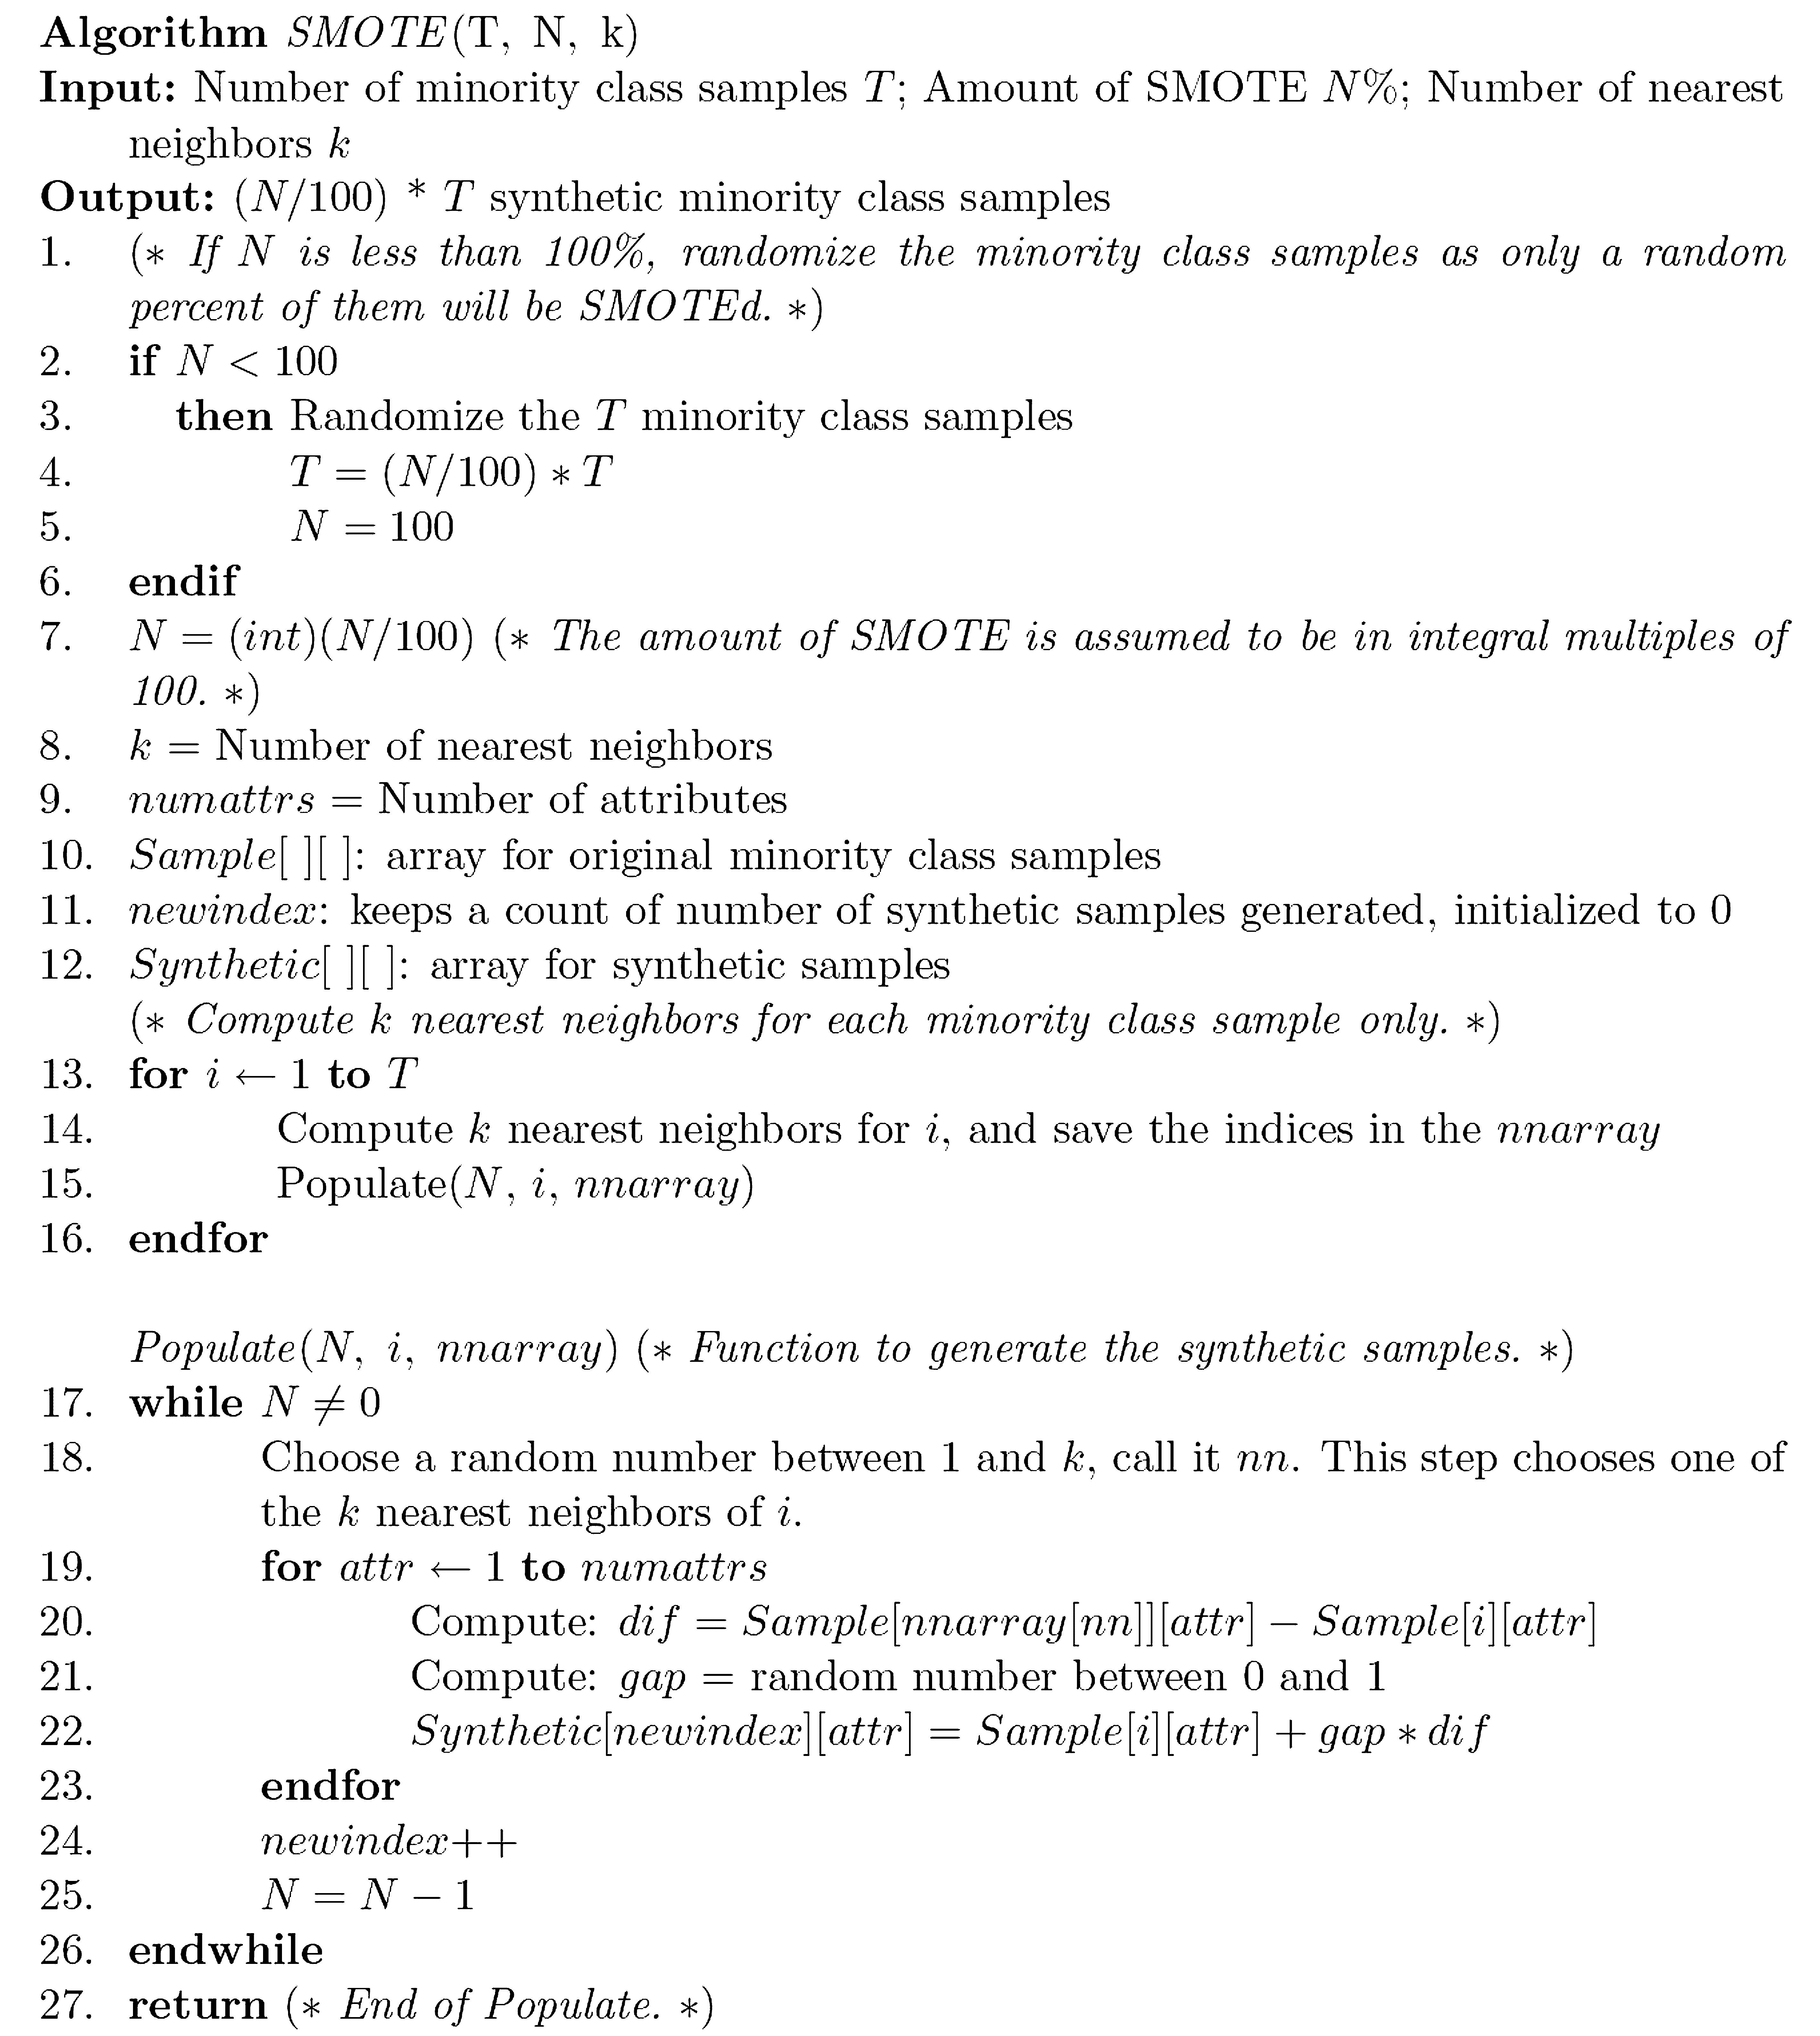
\includegraphics[width=\linewidth]{SMOTE_pseudocode.jpg}
  \end{tabular}
  \caption{Pesudocode for SMOTE}
  \label{alg:smote}
\end{algorithm}

\subsection{Parameter Tuning}
The classifiers (referred to as \textit{predictors} henceforth) being used in this paper are both tree based learners. The recurse on their splits. Their output is a boolean value \texttt{[True/False]}. But make this decision, they use a lot of parameters. Figure~\ref{tbl:parameters} shows all the parameters that matter for defect prediction. In the usual case, the user is expected to supply these values. The goal of {\bfseries RQ2} is simply to use a metaheuristic\footnote{\url{http://en.wikipedia.org/wiki/Metaheuristic}} algorithm to automate this tuning process. There are very many techniques to do this otherwise, without using Metaheuristics, like using gradient
descent optimizers~\cite{salt00}. There are also simpler techniques like Simulated annealing which is often used in search-based SE e.g.~\cite{fea02a,me07f}. Another popular technique is Differential Evolution~\cite{storn97}; there are a lot more methods. 

This paper uses make an engineering decision to use DE. In fact, DEs have been applied before for parameter tuning (e.g. see \cite{chiha12},~\cite{om07}). A recent, as of yet unpublished, paper by Fu et al.~\cite{Fu} also makes a case for DE as a tuner for defect prediction. 

\subsubsection*{Differential Evolution}
The psuedocode for differential evolution is shown in Algorithm~\ref{alg:DE}.
Note that, as the algorithm is described,
any superscript number denotes a line in that algorithm.
DE is an evolutionary algorithm where the next {\em Generation} is learnt from
the current {\em Population}.  If the new is not any better than the current instance, then a \textit{life} is lost (terminating when lives is zero)$^5$.
Each candidate solution in the {\em Population}  
is a pair of {\em (Tunings, Scores)}.  {\em Tunings} are selected from \ref{tbl:parameters} and {\em Scores} come from training a learner using those parameters
and applying it test data$^{23-28}$.

The premise of DE  is that the best way to mutate existing tunings
is to {\em Extrapolate}$^{29}$
between current solutions.  Three solutions $a,b,c$ are selected at random.
For each tuning parameter $i$, at some probability {\em cr}, we replace
the old tuning $x_i$ with $y_i$:
\bi
\item (For numerics) $y_i = a_i+f \times (b_i - c_i)$   where $f$ is a parameter
controlling the cross-over amount.  The {\em trim} function$^{39}$ limits the new
value to the legal range min..max of that parameter.
\item (For booleans) $y_i= \neg x_i$ (see line 37).
\ei
The main loop of DE$^7$ runs over the {\em Population}, replacing old items
with new {\em Candidate}s (if the new candidate is better than the old item).
This means that, as the loop progresses, the {\em Population} is full of increasiningly
more valuable solutions. This, in turn, also improves  the candidates, which are generated
from the {\em Population}.

For the experiments of this paper, we collect performance
values from a data miner, from which a {\em Goal} function extracts one 
performance value$^{27}$ (so this code is rerun many times, each time with
a different {\em Goal}$^2$).  Technically, this makes a  {\em single objective} DE (and for notes on multi-objective DEs, see~\cite{Coello05,zhang07,5583335}).


\begin{algorithm}[htbp!]
  
  \scriptsize
  \begin{algorithmic}[1]
    \Require $\mathit{np} = 10$, $f=0.75$, $cr=0.3$, $\mathit{life} = 5$, $\mathit{Goal} \in \{\mathit{pd},f,...\}$
    \Ensure $S_{best}$
    
    ~\\
    \Function{DE}{$\mathit{np}$, $f$, $cr$, $\mathit{life}$, $\mathit{Goal}$}
    \State $Population  \gets $ $InitializePopulation$($\mathit{np}$)   
    \State $S_{best} \gets $$GetBestSolution$($Population $)
    \While{$\mathit{life} > 0$}
    \State $NewGeneration \gets \emptyset$
    \For{$i=0 \to \mathit{np}-1$}
    \State $S_i \gets$ Extrapolate($Population [i], Population , cr, f$)
    \If {Score($S_i$)$\ge$Score($Population [i]$)}
    \State $NewGeneration$.$append$($S_i$)
    \Else
    \State $NewGeneration$.$append$($Population [i]$)
    \EndIf
    \EndFor
    \State $Population  \gets NewGeneration$
    \If{$\neg$ $Improve$($Population $)}
    \State $life -=1$
    \EndIf
    \State $S_{best} \gets$ $GetBestSolution$($Population $)
    \EndWhile
    \State \Return $S_{best}$
    \EndFunction
    \Function{Score}{$Candidate$}
    \State set tuned parameters according to $Candidate$
    \State $model \gets$$TrainLearner()$
    \State $result \gets$$TestLearner$($model$)   
    \State \Return$\mathit{Goal}(result)$  
    \EndFunction
    \Function{Extrapolate}{$old, pop, cr, f$}
    \State $a, b, c\gets threeOthers(pop,old)$  
    \State $newf \gets \emptyset$
    \For{$i=0 \to \mathit{np}-1$}
    \If{$cr < random()$}
    \State $newf$.$append$($old[i]$)
    \Else
    \If{typeof($old[i]$) == bool}
    \State $newf$.$append$(not $old[i]$)
    \Else
    \State $newf$.$append$(trim($i$,($a[i] + f * (b[i] - c[i]$)))) 
    \EndIf
    \EndIf
    \EndFor
    \State \Return $newf$
    \EndFunction
  \end{algorithmic} 
  \caption{Pesudocode for DE with Early Termination}
  \label{alg:DE}
\end{algorithm}



\section{Data Sets}

The following section describes the experimental rig and the experiments used to measure the performance of the defect predictors on 8 data sets. And, 1 security flaw dataset.

\subsection{Defect Data Set}
The data for defect prediction was obtained from the PROMISE repository\footnote{Promise Repository: \url{http://openscience.us/repo}}. For the defect data, this work investigated 24 releases from 8 open source Java projects. These projects are characterized by the metrics highlighted in figure ~\ref{fig:ck}. The datasets include \emph{Apache Ant} (1.5 -- 1.7), \emph{Apache Camel} (1.2 -- 1.6), \emph{Apache Ivy} (1.1 -- 2.0), \emph{JEdit} (4.1 -- 4.3), \emph{Apache Log4j} (1.0 -- 1.2), \emph{Apache Lucene} (2.0 -- 2.2), \emph{PBeans} (1.0 and 2.0), \emph{Apache POI} (2.0 -- 3.0), \emph{Apache Synapse} (1.0 -- 1.2), \emph{Apache Velocity} (1.4 -- 1.6), and \emph{Apache Xalan-Java} (2.5 -- 2.7). 

Given the empirical nature of the data, it is important to design an experiment such that the prediction phase uses only the \emph{past} data to learn trends which can then be applied to the \emph{future} data. Thus for the experiment data sets that have at least two consecutive releases are used. 
\begin{itemize}
	\item To predict for defects in release $i$, the predictor uses releases releases $(i-1)$ and $(i-2)$.
	\item The tuning uses releases $(i-1)$ and $(i-2)$ to tune. Therein, the paper uses $(i-2)$ as training and $(i-2)$ for testing the scheme.
\end{itemize}

The attributes of the datasets being used have been summarized in figure \ref{fig:attr}.

\begin{figure}[tbp!]
	\renewcommand{\baselinestretch}{1.25}\begin{center}
		{\scriptsize
			\begin{tabular}{l@{~~~}l@{~~~}l@{~~~}l@{~~~}c@{~~~}l@{~~}l@{~~}}
				\hline
				\rowcolor[HTML]{EFEFEF}
				Data & Symbol & Training & Testing & Training& Bugs&\% {\cellcolor[HTML]{EFEFEF}Defective}\\
				\rowcolor[HTML]{EFEFEF}
				 &  & Version & Version & Samples& &\\\hline
				 
				
				Ant & ant & 1.5, 1.6  &1.7 & 644&124&19.25\\
				
				Ivy & ivy & 1.1, 1.4 & 2.0  & 352 & 79 & 22.44\\
				
				Jedit & jed & 4.1, 4.2 & 4.3 & 679 & 127 & 18.70\\
								
				Lucene & luc & 2.0, 2.2 & 2.4 & 442 & 235 & 53.16\\
				
				Poi & poi & 2.0, 2.5 & 3.0 & 699 & 285 & 40.77\\
				
				Synapse & syn & 1.0, 1.1 & 1.2 & 379 & 76 & 20.05\\
				
				Velocity & vel & 1.4, 1.5 & 1.6 & 410& 289 & 70.48\\
				
				Xalan & xal &2.5, 2.6 &2.7 & 1688 & 798 & 47.27\\\hline
			\end{tabular}}
		\end{center}
		\caption{Attributes of the defect data sets}\label{fig:attr}
	\end{figure}


\subsection{Bugzilla Flaw Dataset}

To perform our replication, there is a need to collect a large number of stack traces from the Firefox product. Unfortunately, because of the requirement to use a historical set of traces due to security data availability, we could not make use of Mozilla’s primary stack trace data website, Mozilla Crash Reports\footnote{\url{https://crash-stats.mozilla.com/home/products/Firefox}}. Instead, we made use of the historical dumps\footnote{\url{https://crash-analysis.mozilla.com/crash_analysis/}}. This historical dataset contains a random sampling of stack trace data (approximately 10\% of the crashes seen by the crash reporting system), sorted by day. We performed our analysis on crashes occurring from May 2010 to March 2012 due to the available security data. These dumps do not contain the entirety of the stack trace; rather, only the topmost filename is included in each trace. We further pruned the dataset to only crashes on the first of every month in the time period. In the end, 1,013,770 occurrences of files in stack traces were recorded.

\section{Experimental Setup}
\subsection{The Rig}

The experimental rig is shown in Figure \ref{fig:rig}. It uses an \textit{oracle} to determine weather a certain test case is defective or not. The oracle has 2 components namely, the trainer and the prediction tool. The trainer is either SMOTE, or DE, or both.

\subsection{Statistical Measures} \label{stats}
Let $\{A,B,C,D\}$ denote the
true negatives, 
false negatives, 
false positives, and 
true positives
(respectively) found by a binary detector. 
Certain standard measures can be computed from
$A,B,C,D$: 
{\footnotesize
{\[
	\begin{array}{ll}
	pd=recall=&D/(B+D)\\
	pf=fallout=&C/(A+C)\\ 
	prec=precision=&D/(D+C) \\
	F =&2*pd*prec/(pd + prec)\\
	G =&2*pd*(1-pf)/(1+ pd - pf)
	\end{array}
	\]}}

All the above vary from zero to one. Following this need to be highlighted:
\begin{itemize}
\item For $pf$ (\textit{Fallout}), the {\em better} scores are {\em smaller}.
\item For all other scores, the {\em better} scores are {\em larger}.
\item  {\em prec}, \textit{G}, and {\em F} refer to {\em both} the defect and non-defective modules. This is different to {\em pf} and {\em recall} which only refer to either non-defective or defective modules (repsectively). 
\end{itemize}


In order to assess the performance of the prediction scheme for the defect data set, we use the G measure from above. This measure is particularly useful because it gives a unified number, a combination of recall and fallout, that characterizes the performance of the predictor. 

Notice that G is a harmonic mean of sensitivity and specificity, which are given by:

\noindent\begin{tabular}{p{0.9\linewidth}}
\centering
\begin{tabular}{lll}
Recall& = &{\Large $\frac{\text{Number of true positives}}{\text{Total no. of defective modules}}$}\\
&&\\
& = & probability of a non-defect, given \\
& & that the prediction is negative
\end{tabular}\\[1.25cm]

\begin{tabular}{lll}
	
	specificity& = &{\Large $\frac{\text{Number of true negatives}}{\text{Total non-defective modules}}$}\\
	&&\\
	& = & probability of defect, given \\
	& & that the prediction is positive \\
\end{tabular}\\
\end{tabular}
	
%
%\[
%
%	\begin{aligned}
%	\text{~ ~specificity} & = \frac{\text{number of true negatives}}{\text{total number of non-defective modules}} \\  \\
%	& = \text{probability of non-defect, given that the prediction is negative}
%	\end{aligned}}
%\]

In the context of our application, we want to have both high sensitivity and high specificity at the same time. And is why G is an appropriate measure. Since it is a harmonic mean, it is always less than the least among sensitivity and specificity. Therefore, a high G implies that both sensitivity and specificity are higher than G itself, as a result simplifying the analysis.

In addition to the above, we rank the different variants of the planning scheme to identify the best approach. We make use of the Scott-Knott procedure, recommended by Mittas \& Angelis in their 2013 IEEE TSE paper~\cite{sk}, to compute the ranks. It works as follows: A list of treatments \textit{l} is sorted by the Medianian score. The list \textit{l} is then split into sub-lists m, n in order to maximize the expected value of the differences in the observed performance before and after division. A statistical hypothesis test \textit{H} is applied on the splits \textit{m, n} to check if they are statistically different. If so, Skott-Knott then recurses on each division. 

The research conducted by Shepperd and MacDonell~\cite{shepperd12a}, Kampenes~\cite{kampenes07} and Kocaguenli et al.~\cite{kocharm13}, highlighted that an ``effect size'' in lieu of a mere hypothesis test is required in order to verfiy if two populations are ``significantly'' different. An ICSE'11 paper by Arcuri~\cite{arcuri11} endorsed the use of Vargha and Delaney's A12 effect size for reporting results in software engineering. Thus, for hypothesis testing H in Skott-Knott, we use the A12 test and a non-parametric bootstrap sampling~\cite{efron93}.


\section{Experimental Results}

This section discusses the experimental results for the experiments. In particular, it broken down into 2 experiments. Experiment 1, deals with the defect dataset, an answers \textbf{RQ1, RQ2, and RQ3}, while Experiment 2 deals with the security flaw data set and answers \textbf{RQ4}. The \textbf{Research Questions \textit{(RQs)}} can be found in section \ref{intro}.

\subsection*{Experiment 1: Defect Dataset} \label{exp1}

The defect dataset we prepared as mentioned in the previous section. In total there were 8 datasets. There were 23 columns in each dataset. The first 22 columns each correspond to the CK and OO metrics, highlighted in Figure \ref{fig:ck}. The data is split into training and testing, figure \ref{fig:attr} shows the version used in each data set for this. Following this, each dataset was process with the following treatments:
\begin{itemize}
\item CART was trained with the training data and defects were predicted from the testing data. All statistical measures, see section \ref{stats}, were obtained by comparing the original with the prediction.
\item Likewise, Random Forest was used to do the same process.
\item Differential Evolution was used to tune the attributes of RF and CART. Then the predictions were obtained using the tuned predictors. \\ \textit{Note: tuning was done with only the training dataset, the test dataset remains unseen by the predictors.}
\item Then, for the \textit{untuned} CART and Random Forest, the training data was treated by SMOTE\textit{ing} them and the statistical measures were obtained.
\item Lastly, the predictors were \textit{Tuned} and training data was SMOTE\textit{ed} prior to using the predictors.
 
\end{itemize}

\noindent It is worth mentioning at this point that the above process was repeated more than 20 times for all cases in order to overcome any measurement biases. The results of all the statistical measures are expressed as median and interquartile ranges obtained from the 20 repetitions for each the 8 data, refer to Appendix A.

The results are rather voluminous, with over 10 columns. This makes analysis prohibitively hard. Therefore, as suggested by section \ref{stats}, using only the G scores could aid the analysis. It needs to be reiterated that since the G measure comprises of both the sensitivity and specificity, it summarizes the predictor's ability to predict both defects and non-defects accurately. 

The G scores are summarized in figure \ref{tab:G}. They are presented in a tabular format, with Skott-Knott ranks as the first column, and the quartile charts as the last. \textit{The larger the Rank, the better the Performance}. It needs to be noted that sometimes, two or more treatments are ranked the same even if they are unequal. This is because they are not \textit{statistically different} and they must be treated as equal by the reader.

\begin{figure*}[t!]
    		\begin{minipage}{0.5\linewidth}
    			{\normalsize {\bfseries \noindent ant\\}}
    			{\scriptsize \begin{tabulary}{\linewidth}{|J|J|J|J|J|}
    					\hline
    					\textbf{Rank} & \textbf{Treatment} & \textbf{Median} & \textbf{IQR} & \bigstrut\\\hline
    					1 &  CART(SMOTE) &    59.0  &  3.0 & \quart{0}{9}{9}{-171} \bigstrut\\
    					\hline  2 &           RF &    61.0  &  0.0 & \quart{15}{0}{15}{-171} \bigstrut\\
    					2 &         CART &    63.0  &  0.0 & \quart{21}{0}{21}{-171} \bigstrut\\
    					\hline  3 & CART(SMOTE,Tune) &    67.0  &  0.0 & \quart{34}{0}{34}{-171} \bigstrut\\
    					3 &     RF(Tune) &    68.0  &  2.0 & \quart{34}{6}{37}{-171} \bigstrut\\
    					\hline  4 & RF(SMOTE,Tune) &    70.0  &  1.0 & \quart{43}{3}{43}{-171} \bigstrut\\
    					\hline  5 &   CART(Tune) &    71.0  &  0.0 & \quart{46}{0}{46}{-171} \bigstrut\\
    					5 &    RF(SMOTE) &    71.0  &  1.0 & \quart{46}{3}{46}{-171} \bigstrut\\
    					\hline \end{tabulary}}
    		\end{minipage}
    		\begin{minipage}{0.5\linewidth}
    			{\normalsize {\bfseries ivy\\}}
    			{\scriptsize \begin{tabulary}{\linewidth}{|J|J|J|J|J|}
    					\hline
    					\textbf{Rank} & \textbf{Treatment} & \textbf{Median} & \textbf{IQR} & \bigstrut\\\hline
    					1 &  CART(SMOTE) &    38.0  &  0.0 & \quart{0}{0}{0}{-88} \bigstrut\\
    					1 &   CART(Tune) &    39.0  &  0.0 & \quart{2}{0}{2}{-88} \bigstrut\\
    					1 &     RF(Tune) &    39.0  &  0.0 & \quart{2}{0}{2}{-88} \bigstrut\\
    					\hline  2 &           RF &    46.0  &  7.0 & \quart{2}{17}{19}{-88} \bigstrut\\
    					\hline  3 & RF(SMOTE,Tune) &    54.0  &  6.0 & \quart{35}{14}{38}{-88} \bigstrut\\
    					3 &         CART &    56.0  &  0.0 & \quart{42}{0}{42}{-88} \bigstrut\\
    					3 &    RF(SMOTE) &    56.0  &  0.0 & \quart{42}{0}{42}{-88} \bigstrut\\
    					3 & CART(SMOTE,Tune) &    59.0  &  7.0 & \quart{33}{16}{49}{-88} \bigstrut\\
    					\hline \end{tabulary}}
    		\end{minipage}
    		\vspace{0.3cm}
    		
    		\begin{minipage}{0.5\linewidth}
    			{\normalsize {\bfseries jedit}}
    			
    			{\scriptsize \begin{tabulary}{\linewidth}{|J|J|J|J|J|}
    					\hline
    					\textbf{Rank} & \textbf{Treatment} & \textbf{Median} & \textbf{IQR} & \bigstrut\\\hline
    					1 & CART(SMOTE,Tune) &    60.0  &  11.0 & \quart{0}{15}{15}{-66} \bigstrut\\
    					\hline  2 & RF(SMOTE,Tune) &    66.0  &  1.0 & \quart{22}{1}{23}{-66} \bigstrut\\
    					2 &  CART(SMOTE) &    67.0  &  0.0 & \quart{24}{0}{24}{-66} \bigstrut\\
    					2 &           RF &    67.0  &  0.0 & \quart{24}{0}{24}{-66} \bigstrut\\
    					2 &     RF(Tune) &    67.0  &  0.0 & \quart{24}{0}{24}{-66} \bigstrut\\
    					\hline  3 &    RF(SMOTE) &    69.0  &  0.0 & \quart{27}{0}{27}{-66} \bigstrut\\
    					\hline  4 &   CART(Tune) &    72.0  &  0.0 & \quart{31}{0}{31}{-66} \bigstrut\\
    					\hline  5 &         CART &    85.0  &  0.0 & \quart{49}{0}{49}{-66} \bigstrut\\
    					\hline \end{tabulary}}
    		\end{minipage}
    		\begin{minipage}{0.5\linewidth}
    			{\normalsize {\bfseries lucene}}
    			
    			{\scriptsize \begin{tabulary}{\linewidth}{|J|J|J|J|J|}
    					\hline
    					\textbf{Rank} & \textbf{Treatment} & \textbf{Median} & \textbf{IQR} & \bigstrut\\\hline
    					1 &   CART(Tune) &    53.0  &  0.0 & \quart{0}{0}{0}{-216} \bigstrut\\
    					\hline  2 &  CART(SMOTE) &    57.0  &  0.0 & \quart{16}{0}{16}{-216} \bigstrut\\
    					2 &         CART &    58.0  &  0.0 & \quart{20}{0}{20}{-216} \bigstrut\\
    					\hline  3 &    RF(SMOTE) &    59.0  &  2.0 & \quart{20}{9}{24}{-216} \bigstrut\\
    					3 & RF(SMOTE,Tune) &    59.0  &  1.0 & \quart{20}{4}{24}{-216} \bigstrut\\
    					3 & CART(SMOTE,Tune) &    60.0  &  5.0 & \quart{8}{21}{29}{-216} \bigstrut\\
    					\hline  4 &           RF &    61.0  &  1.0 & \quart{29}{4}{33}{-216} \bigstrut\\
    					\hline  5 &     RF(Tune) &    65.0  &  1.0 & \quart{45}{4}{49}{-216} \bigstrut\\
    					\hline \end{tabulary}}
    		\end{minipage}
    		\vspace{0.3cm}
    		
    		\begin{minipage}{0.5\linewidth}
    			{\normalsize {\bfseries poi}}
    			
    			{\scriptsize \begin{tabulary}{\linewidth}{|J|J|J|J|J|}
    					\hline
    					\textbf{Rank} & \textbf{Treatment} & \textbf{Median} & \textbf{IQR} & \bigstrut\\\hline
    					1 &         CART &    46.0  &  0.0 & \quart{0}{0}{0}{-102} \bigstrut\\
    					\hline  2 &  CART(SMOTE) &    56.0  &  4.0 & \quart{18}{9}{22}{-102} \bigstrut\\
    					2 & CART(SMOTE,Tune) &    56.0  &  6.0 & \quart{18}{13}{22}{-102} \bigstrut\\
    					2 &    RF(SMOTE) &    60.0  &  4.0 & \quart{24}{10}{31}{-102} \bigstrut\\
    					\hline  3 &           RF &    62.0  &  3.0 & \quart{31}{7}{36}{-102} \bigstrut\\
    					3 &   CART(Tune) &    63.0  &  0.0 & \quart{38}{0}{38}{-102} \bigstrut\\
    					3 &     RF(Tune) &    63.0  &  8.0 & \quart{31}{18}{38}{-102} \bigstrut\\
    					\hline  4 & RF(SMOTE,Tune) &    65.0  &  3.0 & \quart{43}{6}{43}{-102} \bigstrut\\
    					\hline \end{tabulary}}
    		\end{minipage}
    		\begin{minipage}{0.5\linewidth}
    			{\normalsize {\bfseries synapse}}
    			
    			{\scriptsize \begin{tabulary}{\linewidth}{|J|J|J|J|J|}
    					\hline
    					\textbf{Rank} & \textbf{Treatment} & \textbf{Median} & \textbf{IQR} & \bigstrut\\\hline
    					1 &     RF(Tune) &    42.0  &  2.0 & \quart{0}{5}{2}{-111} \bigstrut\\
    					\hline  2 &           RF &    45.0  &  0.0 & \quart{11}{0}{11}{-111} \bigstrut\\
    					\hline  3 &  CART(SMOTE) &    48.0  &  0.0 & \quart{19}{0}{19}{-111} \bigstrut\\
    					\hline  4 &         CART &    52.0  &  0.0 & \quart{30}{0}{30}{-111} \bigstrut\\
    					4 &   CART(Tune) &    52.0  &  0.0 & \quart{30}{0}{30}{-111} \bigstrut\\
    					\hline  5 &    RF(SMOTE) &    56.0  &  0.0 & \quart{41}{0}{41}{-111} \bigstrut\\
    					\hline  6 & RF(SMOTE,Tune) &    57.0  &  2.0 & \quart{44}{5}{44}{-111} \bigstrut\\
    					6 & CART(SMOTE,Tune) &    58.0  &  0.0 & \quart{47}{0}{47}{-111} \bigstrut\\
    					\hline \end{tabulary}}
    		\end{minipage}
    		\vspace{0.3cm}
    		
    		
    		\begin{minipage}{0.5\linewidth}
    			{\normalsize {\bfseries velocity}}
    			
    			{\scriptsize \begin{tabulary}{\linewidth}{|J|J|J|J|J|}
    					\hline
    					\textbf{Rank} & \textbf{Treatment} & \textbf{Median} & \textbf{IQR} & \bigstrut\\\hline
    					1 &  CART(SMOTE) &    42.0  &  4.0 & \quart{0}{11}{11}{-102} \bigstrut\\
    					\hline  2 &         CART &    45.0  &  0.0 & \quart{19}{0}{19}{-102} \bigstrut\\
    					\hline  3 & CART(SMOTE,Tune) &    48.0  &  0.0 & \quart{27}{0}{27}{-102} \bigstrut\\
    					3 &   CART(Tune) &    50.0  &  0.0 & \quart{33}{0}{33}{-102} \bigstrut\\
    					\hline  4 &    RF(SMOTE) &    52.0  &  1.0 & \quart{36}{2}{38}{-102} \bigstrut\\
    					4 & RF(SMOTE,Tune) &    52.0  &  3.0 & \quart{33}{8}{38}{-102} \bigstrut\\
    					\hline  5 &     RF(Tune) &    55.0  &  2.0 & \quart{44}{5}{47}{-102} \bigstrut\\
    					5 &           RF &    56.0  &  1.0 & \quart{47}{2}{49}{-102} \bigstrut\\
    					\hline \end{tabulary}}
    		\end{minipage}
    		\begin{minipage}{0.5\linewidth}
    			{\normalsize {\bfseries xalan}}
    			
    			{\scriptsize \begin{tabulary}{\linewidth}{|J|J|J|J|J|}
    					\hline
    					\textbf{Rank} & \textbf{Treatment} & \textbf{Median} & \textbf{IQR} & \bigstrut\\\hline
    					1 &   CART(Tune) &    57.0  &  0.0 & \quart{0}{0}{0}{-215} \bigstrut\\
    					1 &     RF(Tune) &    57.0  &  0.0 & \quart{0}{0}{0}{-215} \bigstrut\\
    					\hline  2 &           RF &    59.0  &  1.0 & \quart{7}{4}{7}{-215} \bigstrut\\
    					2 &  CART(SMOTE) &    60.0  &  3.0 & \quart{3}{12}{11}{-215} \bigstrut\\
    					\hline  3 & CART(SMOTE,Tune) &    64.0  &  6.0 & \quart{11}{23}{26}{-215} \bigstrut\\
    					3 &         CART &    65.0  &  0.0 & \quart{30}{0}{30}{-215} \bigstrut\\
    					\hline  4 &    RF(SMOTE) &    69.0  &  2.0 & \quart{38}{8}{46}{-215} \bigstrut\\
    					4 & RF(SMOTE,Tune) &    69.0  &  1.0 & \quart{46}{3}{46}{-215} \bigstrut\\
    					\hline \end{tabulary}}
    		\end{minipage}

\caption{G-Scores for the Defect Prediction Datasets}
\label{tab:G}
\end{figure*}

{\textbf{RQ1:  Can over/under sampling techniques such as SMOTE to improve prediction accuracy for defect prediction?} \textit{Yes.}}

In 6 out of the 8 datasets, RF proved to be better than CART as was reported by Lessmann et al. \cite{lessmann}.
In 4 out of the 6 datasets where RF was the better predictor, SMOTE\textit{ing} ranked better than raw training data. Thus, \textit{SMOTEing does improve prediction accuracy} 

{{\bfseries RQ2: Does Tuning a data miner improve it's prediction accuracy?} \textit{Not always. Works in only a few datasets.}}


Just tuning the predictor seems only to help in 4 out of the 8 datasets. This was to be expected however because merely tuning a predictor is not going to change the nature of the dataset. If the dataset is skewed, it is going to pose the same problem to the predictor regardless of it being tuned or not. 

With respect to the 4 datasets where it does work, there is a possibility that the data is not only skewed other factors affect the prediction accuracy. And this needs to be studied.

{{\bfseries RQ3: Is tuning performed in conjunction with SMOTE any better than either one performed alone?}\textit{Yes.}}

This is a particularly interesting result. In 5 out of the 8 dataset, the use of both as beneficial. In ant RF+SMOTE+Tune is almost as good as RF+SMOTE, and definitely better than plain RF. Similarly, in ivy, poi, synapse and xalan the results hold true. 

Note that, with the exception of jedit, using tools such as DE and SMOTE to prepare both the predictor and the training data is beneficial.


\begin{figure}[t!]
	{\normalsize \textbf{Before SMOTE:}\\[0.1cm]
	\begin{tabulary}{\linewidth}{JJJJJ}
				
		\rowcolor[HTML]{DFDFDF}
		\cellcolor[HTML]{EFEFEF}Rank & \cellcolor[HTML]{EFEFEF}Name        & \cellcolor[HTML]{EFEFEF}Median   & \cellcolor[HTML]{EFEFEF}IQR  & \\ 
		1    & Accuracy    & 99.00 & 2.00 & \quart{48}{2}{48}{100}  \bigstrut\\
		1    & Recall      & 100.00 & 3.00 & \quart{49}{3}{49}{100} \bigstrut\\
		1    & \textbf{Specificity} & \textbf{8.00} & \textbf{4.00} & \quart{2}{4}{4}{100} \bigstrut\\
		1    & Precision   & 99.00 & 3.00 & \quart{48}{3}{48}{100} \bigstrut\\
		1    & F           & 100.00 & 2.00 & \quart{49}{3}{49}{100} \bigstrut\\
		1    & \textbf{G}           & \textbf{15.00} & \textbf{3.00} & \quart{6}{3}{7}{100} \bigstrut\\[0.2cm] 
	\end{tabulary}}
		\vspace{3pt}
		{\normalsize \textbf{After SMOTE:}\\
			\begin{tabulary}{\linewidth}{JJJJJ}
				
				\rowcolor[HTML]{DFDFDF}
				\cellcolor[HTML]{EFEFEF}Rank & \cellcolor[HTML]{EFEFEF}Name        & \cellcolor[HTML]{EFEFEF}Median   & \cellcolor[HTML]{EFEFEF}IQR  & \\ 
				1    & Accuracy    & 80.00 & 2.00 & \quart{39.5}{2}{40}{100}  \bigstrut\\
				1    & Recall      & 77.00 & 3.00 & \quart{38}{3}{38.5}{100} \bigstrut\\
				1    & \textbf{Specificity }& \textbf{81.00} & \textbf{4.00} & \quart{39.5}{4}{41}{100} \bigstrut\\
				1    & Precision   & 78.00 & 3.00 & \quart{38.5}{3}{39}{100} \bigstrut\\
				1    & F           & 77.00 & 2.00 & \quart{38.5}{3}{38.5}{100} \bigstrut\\
				1    & \textbf{G}           & \textbf{80.00} & \textbf{3.00} & \quart{39}{3}{40}{100} \bigstrut\\
			\end{tabulary}}
	\caption{Performance Scores Before and After SMOTE for the Bugzilla Security Flaw Dataset} \label{bugzilla}
\end{figure}

\subsection{Experiment 2: Bugzilla Secturity Flaw Dataset}

This was one contiguous data set with 60000 instance of which only 391 were security flaws. This a classic example of skewness in the data.

Since there is only one dataset in this category, this paper tested the statistical validity of the predictors by performing a 5$\times$5 cross validation study. For this, the data was randomly grouped into sets of 5, one of the set was used as testing and other 4 are used as training, then the same is repeated for the 4 remaining datasets. This entire process is repeated 5 more times. Therefore, a total of 25 evaluations of the stats are performed. They are then tabulated using the median and interquartile spread.

Although the SMOTE algorithm was applied to this dataset, it was slightly altered to fit the application. In usual SMOTE, as previously discussed, minority classes are synthetically oversampled and the majority class is randomly undersampled by a certain fraction. Due to the nature of the minority class in this dataset, it was reasoned that creating new rows would translate to inserting artificial security flaw which might not be fair. Therefore, for this dataset, only the majority class was under sampled and the minority class was unaltered. Moreover, it was ensured that the number of majority and minority class samples are the same.

{{\bfseries RQ4: Can SMOTE\textit{ing} technique be applied to other Software Engineering paradigms?} Yes.}


As was reported in the previous papers, a simple Random Forest on the dataset without any sort of preprocessing produce true appalling results, see Figure \ref{bugzilla}.

However, once the data was preprocessed by undersampling the majority class, the prediction performance improved drastically. In fact, the specificity, which measures the probability of security flaw given the predictor tests positive, rose from just 0.08 (80\%) before sampling to 0.81 (81\%) after sampling. That's an order of magnitude better. 
 
\section{Conclusions}

This work has shown that the use of off-the-shelf predictors is not a wise approach for software defect prediction. The results show that one must reflect on the nature of the data they are handling and the reason a specific predictor is being used. In general, result have seem to conclude that one of the tree based classifier RF is better than the other. In addition, use of a preprocessing tool to prepare the dataset and a mechanism to determine the attributes of a classifier are important. More importantly, the use of both in general is also quite beneficial. It is true that the data sets being handled here are open-source projects that may not have adhered to any strict development strategy, this adds another dimension to what causes defects. This can't be handled by machine learning. It is therefore advisable that one conduct as test such as this to see what the best approach to defect prediction. A strong statistical reasoning is also pertinent to making managerial decision regarding a project.

Another purpose of this paper was to test if the sampling helps improve security flaws. The results are very positive and further affirm the need for data preprocessing before any sort of predictive analytics is performed.

\section*{Acknowledgments}

The author would like to thank Mr. Chris Theisen for providing the Bugzilla security flaw dataset. 

\bibliographystyle{IEEEtran}
\bibliography{Ref}

\newpage
\appendices
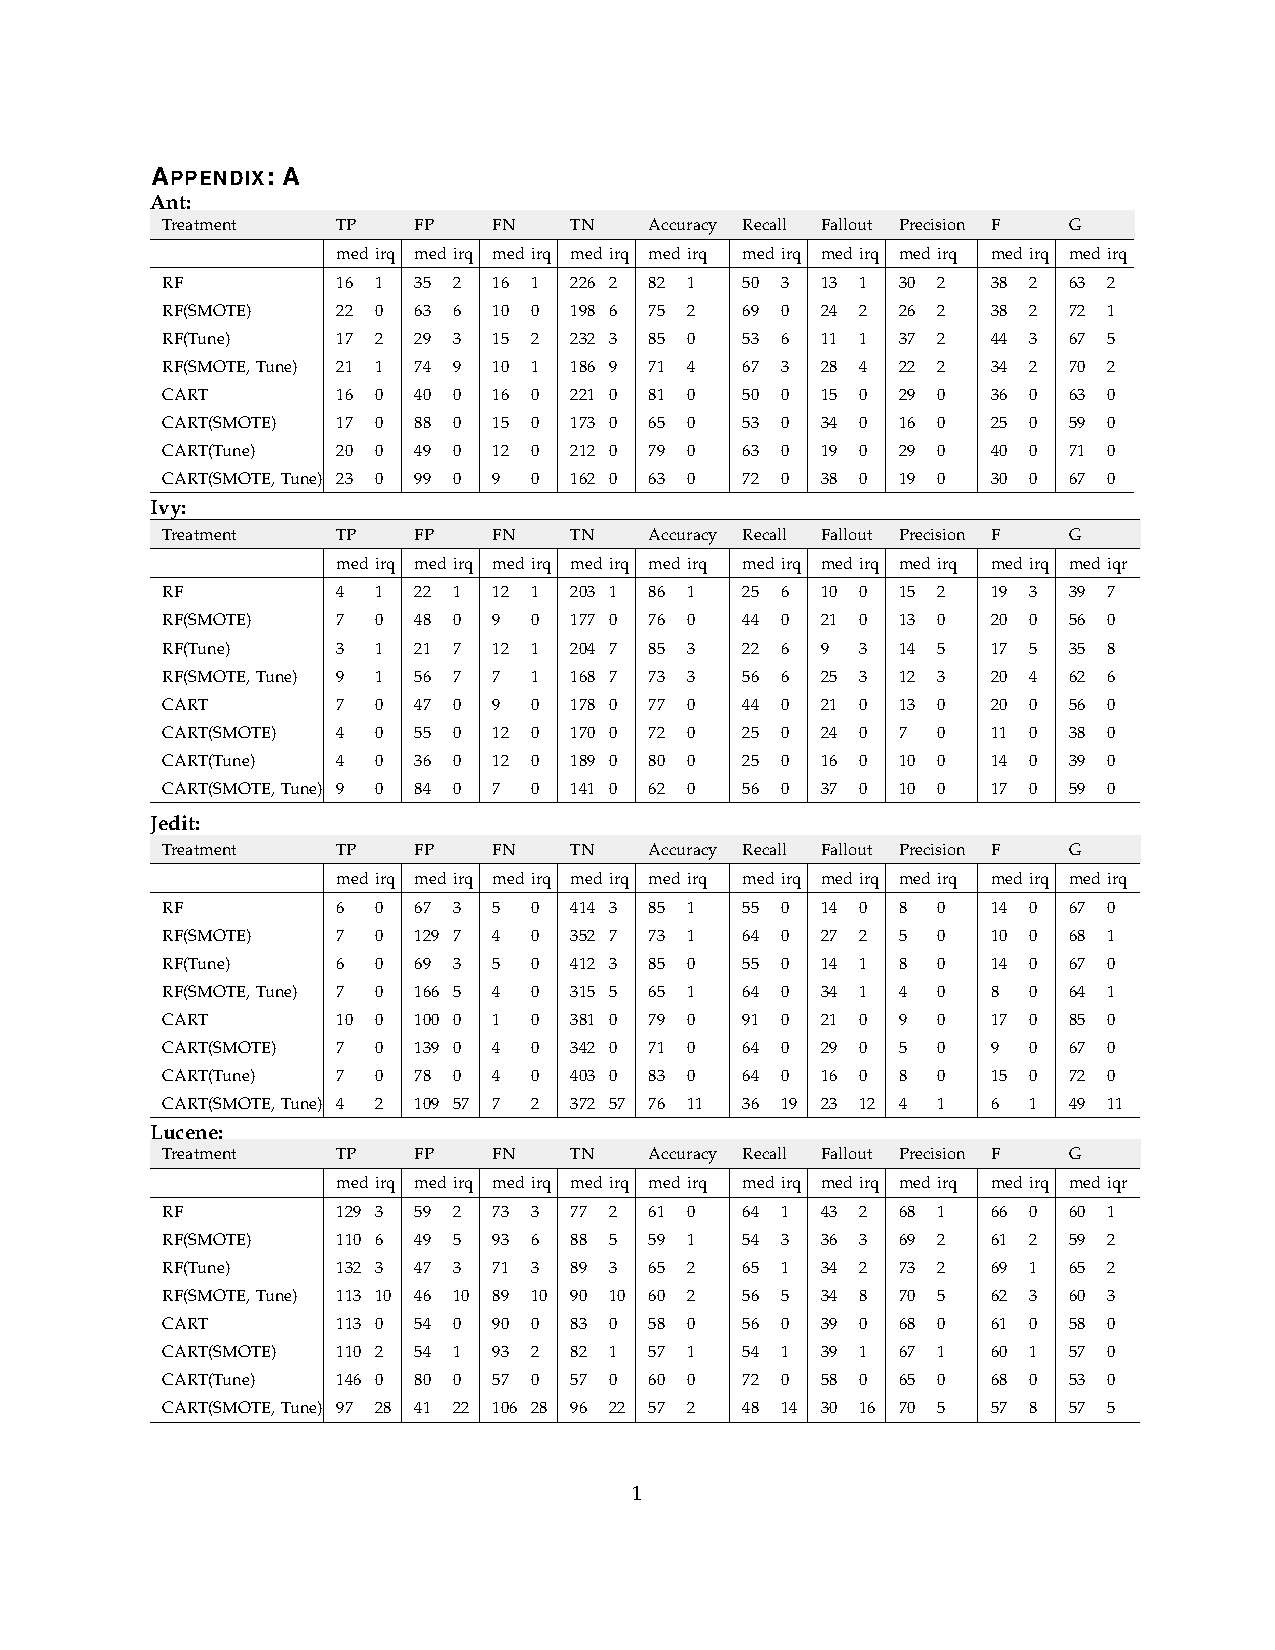
\includepdf[pages={1,2}]{Appendix.pdf}

\newpage

\end{document}